\documentclass[11pt]{article}
\usepackage[margin=1in]{geometry}
\usepackage[T1]{fontenc}
\usepackage{lmodern}
\usepackage{microtype}
\usepackage{amsmath}
\usepackage{booktabs}
\usepackage{graphicx}
\usepackage{caption}
\usepackage{subcaption}
\usepackage[hidelinks]{hyperref}
\graphicspath{{figures/}}
\captionsetup{font=small,labelfont=bf}
\setlength{\parskip}{0.4em}

\title{\textbf{Lane Marker Detection with a Spatial CNN}}
\author{Cooper Malone\\University of Nebraska--Lincoln}
\date{}

\begin{document}
\maketitle

\begin{abstract}
\noindent
Lane markings are hard to segment because they are thin and long, and traffic, shadows and glare
often hide parts of them. This project implements a Spatial CNN (SCNN), which passes information
across the rows and columns of a feature map so that a lane line can stay continuous where part of
it is hidden. The model uses a ResNet-18 backbone and is trained on the CULane dataset to predict a
binary lane mask. Training ran in two phases on a single V100 GPU: 48 epochs on a 2{,}000-image
subset, then 48 epochs on the full 88{,}880-image training set. On the full validation set, the
model reached its best IoU of 0.297 and F1 of 0.441 after only 12 epochs on the subset. Training on
44 times more data never improved on this (best IoU 0.295, F1 0.437), and validation loss rose
steadily in both phases while IoU and F1 held flat. The analysis traces this plateau to the model's
output resolution. Message passing runs on a $9\times25$ feature grid, one cell per $32\times32$
pixels, and the result is upsampled 32 times. The predicted masks therefore find the lanes but are
much wider than the painted lines, which caps IoU whatever the amount of data. The report closes with
the changes this diagnosis points to, chiefly computing features at one-eighth resolution.
\end{abstract}

\section{Introduction}

Lane detection underlies lane keeping, lane departure warning and the localization and path
planning of autonomous vehicles. The task is to find the lane markings painted on the road in an
image from a forward-facing camera. Lane markings are a difficult segmentation target: they are
thin, they stretch across most of the image, and in city traffic they are often worn, hidden by
vehicles, shadowed, or washed out by glare. A standard segmentation network decides each pixel from
a local neighborhood, so where a marking is hidden it tends to lose the line.

The Spatial CNN~\cite{pan2018} addresses this by passing messages slice by slice across a feature
map: each row receives information from the row above it, each column from its neighbor, and so on
in four directions. Evidence of a lane at one end of the image can then reach the other end, which
suits long, continuous structures.

This project implements an SCNN-style network on a ResNet-18 backbone, trains it on the CULane
benchmark~\cite{pan2018} on a GPU cluster, and analyzes where its performance is limited. The main
findings are that the model learns lane positions quickly, that more training data does not improve
it, and that its output resolution, not its data, sets the ceiling.

\section{Related Work}

Classical lane detectors find edges with filters such as the Canny detector and fit lines or curves
with the Hough transform. They work on clear highways but fail under occlusion, shadows and worn
paint. Deep segmentation networks learn the task from labeled images instead; encoder--decoder
models with atrous convolutions such as DeepLabv3+~\cite{chen2018} are a common general-purpose
choice for dense prediction.

Pan et al.~\cite{pan2018} introduced both SCNN and the CULane dataset. Their network applies
slice-by-slice convolutions in four directions to a feature map at one-eighth of the input
resolution and predicts a separate probability map for each of up to four lanes. Hou et
al.~\cite{hou2019} obtained similar accuracy with a lighter network through self-attention
distillation. TuSimple~\cite{tusimple2017} (highway driving) and BDD100K~\cite{yu2020} (diverse
driving scenes) are other widely used datasets, and Al Mamun et al.~\cite{mamun2022} survey deep
learning methods for lane detection.

\section{Method}

\subsection{Task}

Each input is an RGB image resized to $288\times800$ pixels. The target is a binary mask $y$ of the
same size in which lane-marking pixels are 1 and all other pixels are 0. All lanes share one class.
This is simpler than the original SCNN, which predicts each lane in its own channel and also predicts
whether each lane exists.

\subsection{Architecture}

The network has four stages.
\begin{enumerate}
  \item \textbf{Backbone.} An ImageNet-pretrained ResNet-18 produces its last feature map (C5) at
        stride 32: 512 channels on a $9\times25$ grid for a $288\times800$ input.
  \item \textbf{Reduction.} A $3\times3$ convolution with batch normalization and ReLU reduces the
        features to 128 channels.
  \item \textbf{Spatial message passing.} The feature map is cut into slices, columns for the
        horizontal sweeps and rows for the vertical ones. Moving slice by slice, each slice receives
        a message from the slice before it, which has already been updated:
        \[
          s'_1 = s_1, \qquad s'_k = s_k + W * \operatorname{ReLU}(s'_{k-1}), \quad k = 2,\dots,n,
        \]
        where $W$ is a $1\times1$ convolution. The map is swept left to right, right to left, top to
        bottom and bottom to top, sharing $W$ across all four sweeps, and is then batch-normalized.
        The updates are written without in-place operations so that automatic differentiation can
        track them.
  \item \textbf{Head.} A $3\times3$ refinement convolution and a $1\times1$ convolution produce one
        logit per grid cell, and bilinear interpolation upsamples the logits by a factor of 32 to the
        input size.
\end{enumerate}
This design departs from Pan et al.\ in three ways that matter later: message passing runs at
stride 32 instead of stride 8, its kernel spans one cell instead of nine, and one kernel is shared by
all four directions.

\subsection{Loss}

The loss adds binary cross-entropy, which scores each pixel, to the Dice loss, which scores the
overlap of the whole predicted region and is less affected by the rarity of lane pixels. With
predicted probabilities $p_i = \sigma(z_i)$ for logits $z_i$,
\[
  \mathcal{L} = -\frac{1}{N}\sum_i \bigl[y_i\log p_i + (1-y_i)\log(1-p_i)\bigr]
  \;+\; 1 - \frac{2\sum_i p_i y_i}{\sum_i p_i + \sum_i y_i}.
\]

\subsection{Metrics}

A pixel is predicted as lane when $p_i > 0.5$. For each validation image, IoU is
$\mathrm{TP}/(\mathrm{TP}+\mathrm{FP}+\mathrm{FN})$ over lane pixels and F1 is
$2\mathrm{TP}/(2\mathrm{TP}+\mathrm{FP}+\mathrm{FN})$; both are averaged over images. These are
pixel-level scores. They are not comparable to the official CULane F1, which matches whole predicted
lanes to annotated lanes, and on which Pan et al.\ report 71.6.

\section{Experimental Setup}

\textbf{Data.} CULane contains 133{,}235 frames from about 55 hours of driving in Beijing, split into
88{,}880 training, 9{,}675 validation and 34{,}680 test images~\cite{pan2018}. The scenes include
heavy traffic, night, shadows, glare, curves and crossroads. Annotated lanes were rasterized into
binary masks. Images were resized to $288\times800$ and normalized with ImageNet statistics, and masks
were resized with nearest-neighbor interpolation. The only augmentation was a random horizontal flip
with probability 0.5.

\textbf{Training.} The model was trained with AdamW (learning rate $10^{-3}$, weight decay $10^{-4}$),
batch size 8 (4 when GPU memory ran short), and automatic mixed precision, on one NVIDIA V100 (32 GB)
of the university's Swan cluster, using SLURM batch jobs limited to 48 hours each. Long runs resumed
from saved checkpoints. The checkpoints held only the model weights, so the optimizer's moment
estimates restarted at each resume. Training ran in two phases:
\begin{itemize}
  \item \textbf{Phase 1}, epochs 1--48: a subset of about 2{,}000 training images, to debug the
        pipeline quickly;
  \item \textbf{Phase 2}, epochs 49--96: the full 88{,}880-image training set, continuing from the
        Phase 1 weights.
\end{itemize}

\textbf{Evaluation.} Every Phase 1 checkpoint was re-evaluated on the full validation list after
training, and Phase 2 was evaluated on the same list after every epoch, so the two phases are
directly comparable.

\section{Results}

\subsection{Quantitative results}

\begin{table}[h]
\centering
\small
\begin{tabular}{lccccc}
\toprule
Phase & Epochs & Training images & Best IoU (epoch) & Best F1 (epoch) & Validation loss \\
\midrule
1 & 1--48  & $\approx$2{,}000 & \textbf{0.297} (12) & \textbf{0.441} (12) & 0.74 $\rightarrow$ 0.93 \\
2 & 49--96 & 88{,}880         & 0.295 (76)          & 0.437 (76)          & 0.86--1.12, rising \\
\bottomrule
\end{tabular}
\caption{Validation results on the full CULane validation set. Phase 1 ended at IoU 0.288 and F1
0.429. In Phase 2, IoU stayed between 0.283 and 0.295 apart from one dip.}
\label{tab:results}
\end{table}

Table~\ref{tab:results} summarizes both phases. In Phase 1 (Figure~\ref{fig:phase1}), IoU and F1 rose
to about 0.29 and 0.43 within two epochs, peaked at epoch 12 and then stayed between 0.279 and 0.297.
Validation loss reached its minimum of 0.73 at epoch 7 and then climbed to 0.93 by epoch 48.

\begin{figure}[h]
\centering
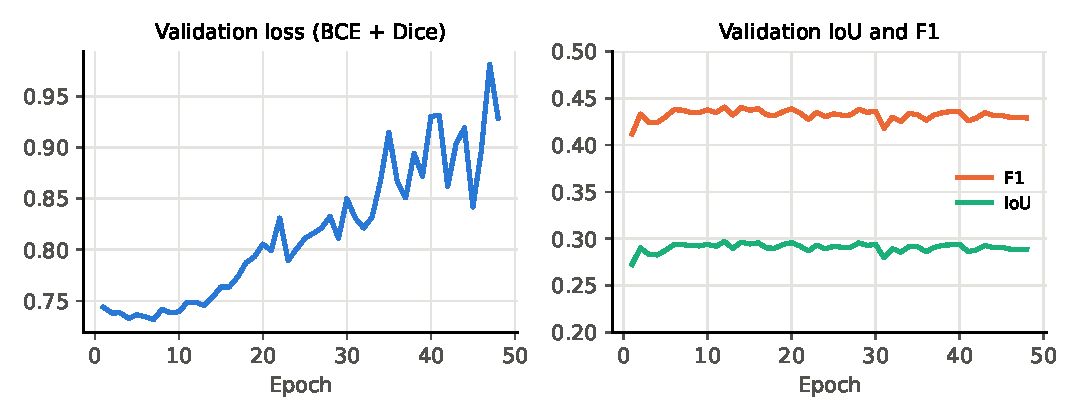
\includegraphics[width=0.95\textwidth]{phase1_metrics.pdf}
\caption{Phase 1, epochs 1--48 on the 2{,}000-image subset, evaluated on the full validation set.
Validation loss rises after epoch 7 while IoU and F1 stay flat.}
\label{fig:phase1}
\end{figure}

Switching to the full training set in Phase 2 (Figure~\ref{fig:phase2}) did not change this
picture. IoU and F1 stayed in the same band, with the best epoch (76) at IoU 0.295 and F1 0.437,
slightly below the Phase 1 peak. Validation loss continued to drift upward, from about 0.93 to about
1.05, with large swings between epochs. At epoch 58, IoU and F1 dropped to 0.25 and 0.38 for a single
epoch, while validation loss reached its lowest Phase 2 value.

\begin{figure}[h]
\centering
\begin{subfigure}{0.49\textwidth}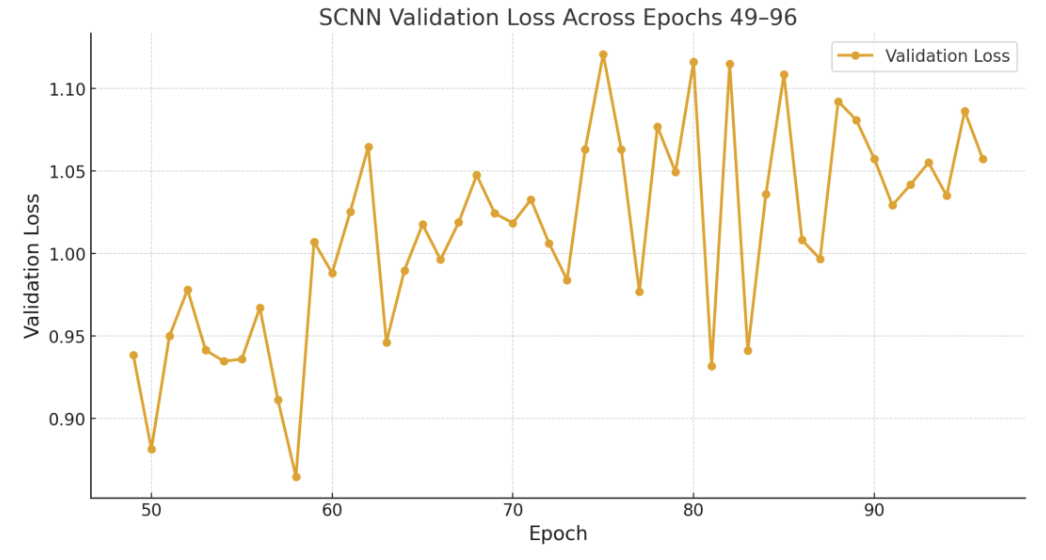
\includegraphics[width=\linewidth]{phase2_loss.png}\caption{Validation loss}\end{subfigure}\hfill
\begin{subfigure}{0.49\textwidth}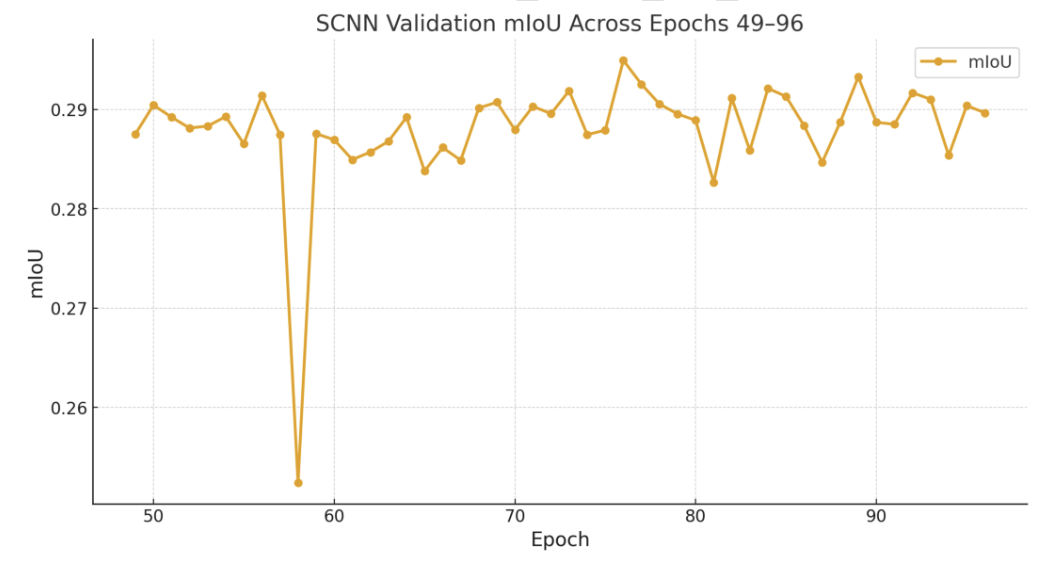
\includegraphics[width=\linewidth]{phase2_iou.png}\caption{IoU}\end{subfigure}\\[4pt]
\begin{subfigure}{0.49\textwidth}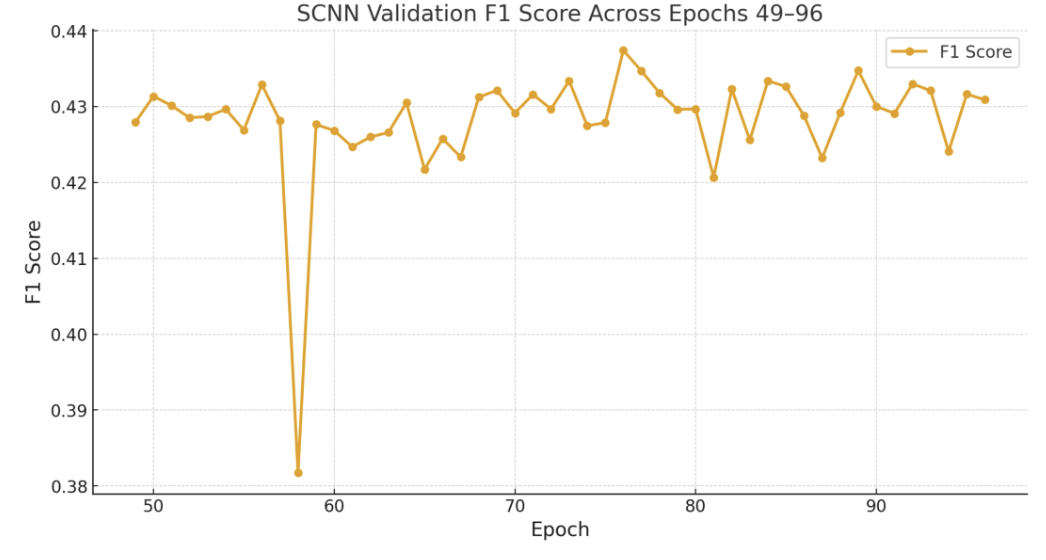
\includegraphics[width=\linewidth]{phase2_f1.png}\caption{F1}\end{subfigure}
\caption{Phase 2, epochs 49--96 on the full training set. IoU and F1 stay near 0.29 and 0.43
while validation loss drifts upward.}
\label{fig:phase2}
\end{figure}

\subsection{Qualitative results}

Figure~\ref{fig:success} shows predictions at epoch 96 on typical urban scenes. The model finds the
lanes, including lanes partly hidden by cars and buses, and the predicted regions follow the lanes'
direction toward the vanishing point. The masks are, however, much wider and wavier than the painted
lines, and most frames show false positives along the bottom edge of the image, on the car's hood.
Figure~\ref{fig:failure} shows typical failures: haze or glare on the windshield washes out the
markings, and the predicted lanes break into fragments.

\begin{figure}[h]
\centering
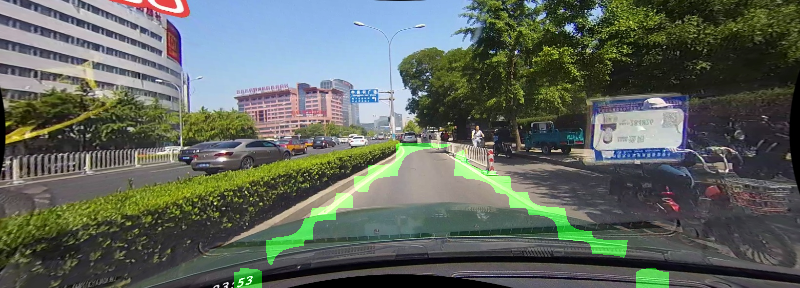
\includegraphics[width=0.48\textwidth]{success_10.png}\hfill
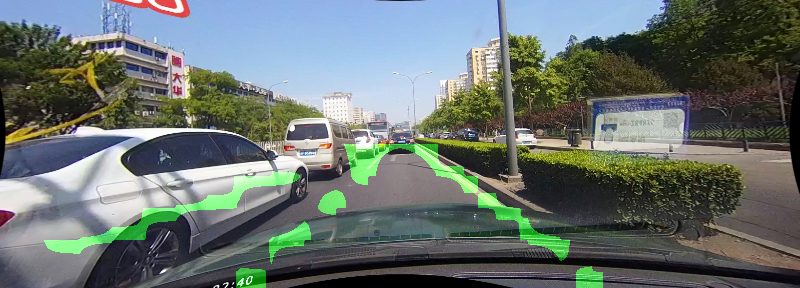
\includegraphics[width=0.48\textwidth]{success_11.png}\\[4pt]
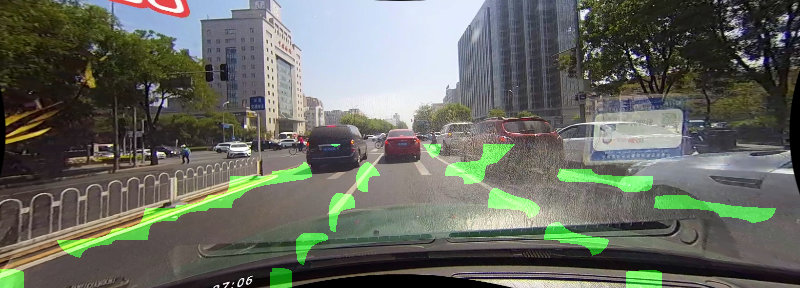
\includegraphics[width=0.48\textwidth]{success_12.png}\hfill
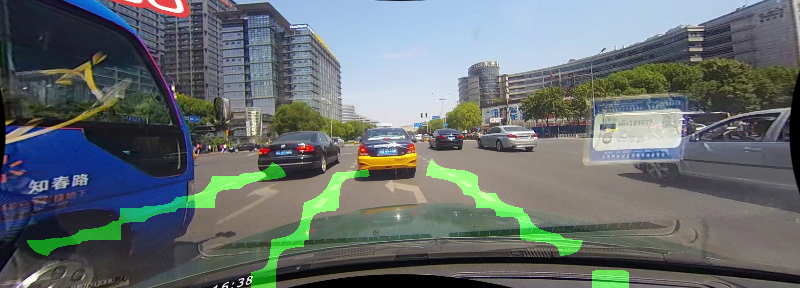
\includegraphics[width=0.48\textwidth]{success_13.png}
\caption{Predicted lane masks (green) at epoch 96. Lane positions and directions are correct, even
next to large vehicles, but the masks are several times wider than the markings.}
\label{fig:success}
\end{figure}

\begin{figure}[h]
\centering
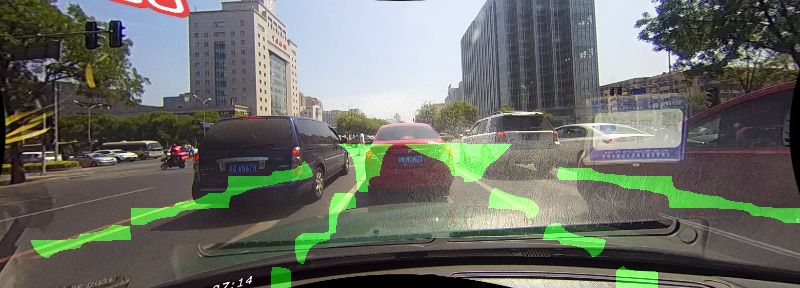
\includegraphics[width=0.48\textwidth]{failure_1.png}\hfill
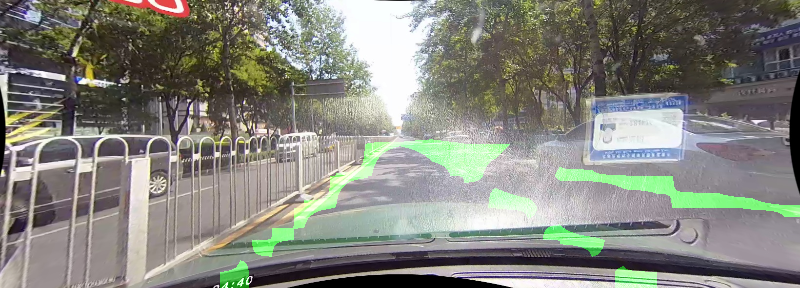
\includegraphics[width=0.48\textwidth]{failure_2.png}
\caption{Failure cases at epoch 96. Haze and glare on the windshield wash out the markings and
fragment the predicted lanes.}
\label{fig:failure}
\end{figure}

\section{Discussion}

\paragraph{More data did not help.} The most informative result is the comparison between the
phases. A model that had seen only 2{,}000 training images reached its best validation score
within 12 epochs, and 48 further epochs on 44 times as much data did not improve on it. When added
data leaves validation accuracy unchanged, the limit is usually the model rather than the data.

\paragraph{The output resolution sets the ceiling.} The architecture explains that limit. Message
passing and the prediction head work on the stride-32 feature map, a $9\times25$ grid in which each
cell covers $32\times32$ input pixels. Bilinear upsampling of this coarse map cannot draw a line a few
pixels wide: every predicted lane is at least about one cell wide, which is the wide, wavy shape in
Figure~\ref{fig:success}. The extra width counts as false positives on every image, so IoU stays
low even when the lane positions are right. The coarse grid also limits SCNN's own benefit, since
there are only 25 columns and 9 rows for messages to travel along. Pan et al.\ apply message passing
at stride 8 ($36\times100$ for this input) with kernels nine cells wide, which keeps lanes thin and
gives messages much more room to propagate.

\paragraph{Rising loss with flat metrics.} In both phases the validation loss rose while IoU and F1
held steady. The thresholded metrics only change when a pixel crosses 0.5, but cross-entropy keeps
growing as the model becomes more confident on the pixels it gets wrong. This is a sign of
overfitting. It began early, after epoch 7, because the Phase 1 subset was so small, and the full
data in Phase 2 did not reverse it. Restarting the optimizer state at each resume may have added to
the large swings in Phase 2.

\paragraph{The epoch-58 dip.} The validation set is the same at every epoch, so the one-epoch drop in
IoU and F1 cannot come from harder images. It reflects the weights at that epoch. Because the loss
reached its lowest Phase 2 value at the same time, the most likely explanation is that the model
became more conservative: fewer pixels crossed the 0.5 threshold, which lowered IoU and F1 while
making the probability-based loss smaller. The next epoch returned to the usual range.

\paragraph{Failure modes.} Glare and windshield haze remove the contrast that marks a lane, and the
only augmentation was a horizontal flip, so the model never saw brightness or contrast changes in
training. The false positives on the hood suggest the model has not learned to ignore the image
region below the road.

\section{Conclusion and Future Work}

The project built a working SCNN-style lane segmentation pipeline and trained it at scale on a GPU
cluster. The model reliably finds lane positions in difficult urban scenes, but its accuracy
plateaued at IoU 0.30 and F1 0.44 after 12 epochs on 2{,}000 images, and 44 times more data did not
move that plateau. The analysis points to the stride-32 output resolution as the main limit. The next
steps, in order of expected impact, are:
\begin{enumerate}
  \item compute features at stride 8, by dilating the last two ResNet stages or adding an FPN-style
        decoder, and run message passing there with wider, direction-specific kernels;
  \item predict each lane in its own channel and evaluate with the official CULane metric, so the
        results can be compared with published work;
  \item add brightness, contrast and glare augmentation, and mask out the car's hood;
  \item save optimizer state in checkpoints, add a learning-rate schedule, and stop early on
        validation loss.
\end{enumerate}

\begin{thebibliography}{9}
\small
\bibitem{mamun2022} A.~Al Mamun, P.~P.~Em, M.~J.~Hossen, A.~Tahabilder and B.~Jahan. A comprehensive
review on lane marking detection using deep neural networks. \emph{Sensors}, 22(19):7366, 2022.

\bibitem{chen2018} L.-C.~Chen, Y.~Zhu, G.~Papandreou, F.~Schroff and H.~Adam. Encoder-decoder with
atrous separable convolution for semantic image segmentation. In \emph{European Conference on
Computer Vision (ECCV)}, pages 833--851, 2018.

\bibitem{hou2019} Y.~Hou, Z.~Ma, C.~Liu and C.~C.~Loy. Learning lightweight lane detection CNNs by
self attention distillation. In \emph{IEEE/CVF International Conference on Computer Vision (ICCV)},
pages 1013--1021, 2019.

\bibitem{pan2018} X.~Pan, J.~Shi, P.~Luo, X.~Wang and X.~Tang. Spatial as deep: Spatial CNN for
traffic scene understanding. In \emph{AAAI Conference on Artificial Intelligence}, volume~32, 2018.

\bibitem{tusimple2017} TuSimple. TuSimple lane detection challenge dataset, 2017.

\bibitem{yu2020} F.~Yu, H.~Chen, X.~Wang, W.~Xian, Y.~Chen, F.~Liu, V.~Madhavan and T.~Darrell.
BDD100K: A diverse driving dataset for heterogeneous multitask learning. In \emph{IEEE/CVF Conference
on Computer Vision and Pattern Recognition (CVPR)}, 2020.
\end{thebibliography}

\end{document}
